\documentclass{article}

\usepackage{graphicx}
\graphicspath{ {./images/} }

\title{Ch. 34 Solutions}
\author{Principles of Macroeconomics}
\date{\today}

\begin{document}

\maketitle

\section*{Quick Quiz}

\begin{enumerate}

\item (c) -- A recession is a period when the economy contracts. That means production -- a.k.a. real GDP -- falls. When firms cut back production, they tend to lay off workers, so unemployment increases.

\item (d) -- Recessions are unpredictable, so they occur irregularly. 

\item (c) -- According to classical macroeconomic theory, the money supply doesn't affect real variables. The GDP deflator measures the price level which is a nominal variable.

\item (a) -- In the short run, the money supply affects real variables.

\item (b) -- Aggregate demand and aggregate supply relate output and the price level.

\item (b) -- A fall in the price level decreases the need for people to hold money. Instead, they lend out more of their money which shifts the supply of loanable funds to the right and increases investment. An increase in investment increases aggregate demand.

\item (d) -- The first two would both decrease consumption, and the third decreases government purchases. That means all three decrease aggregate demand at any given price level.

\item (d) -- If wages are sticky, that means nominal wages are fixed in the short run. When the price level increases, the real value of those nominal wages decreases. If real wages decrease, then firms' costs decrease. Therefore, firms produce more. A higher price level leads to increased production. In other words, the supply curve slopes up.

\item (d) -- The other three options would also shift LRAS. 

\newpage

\item (c) -- Business pessimism will decrease investment. That shifts AD left which leads to lower output.

	\begin{center}
	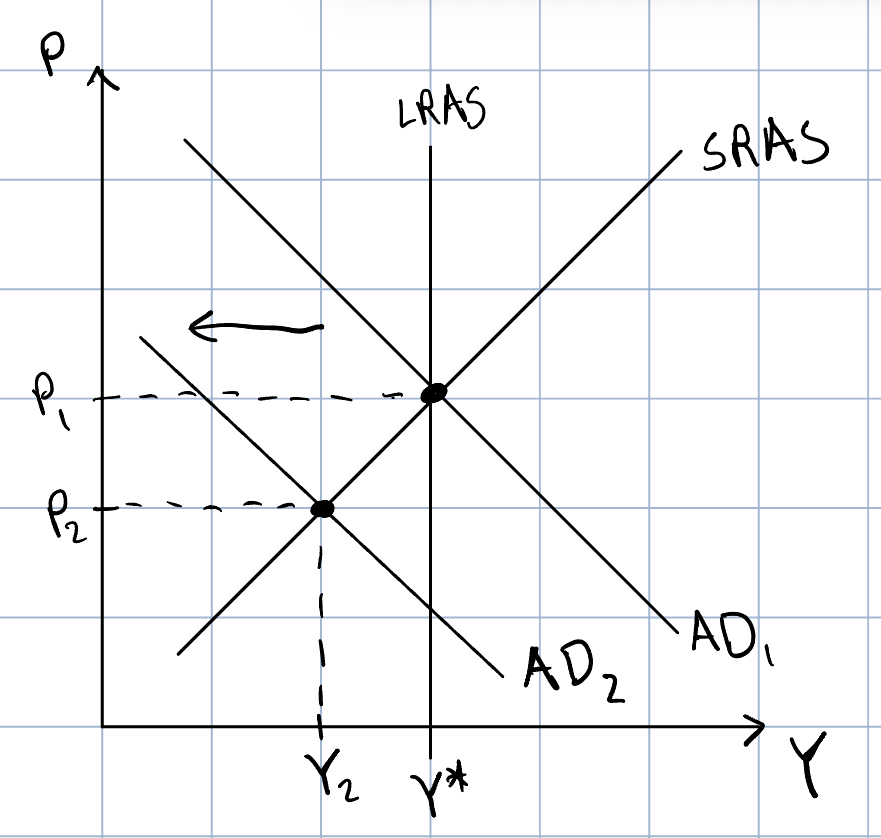
\includegraphics[width = 0.4\textwidth]{qq10}
	\end{center}
	
\item (a) -- In the short run, output increases, but in the long run, output returns to its natural level when SRAS shifts left. In the short run price level increases, but in the long run, price level increases further when SRAS shifts left.

	\begin{center}
	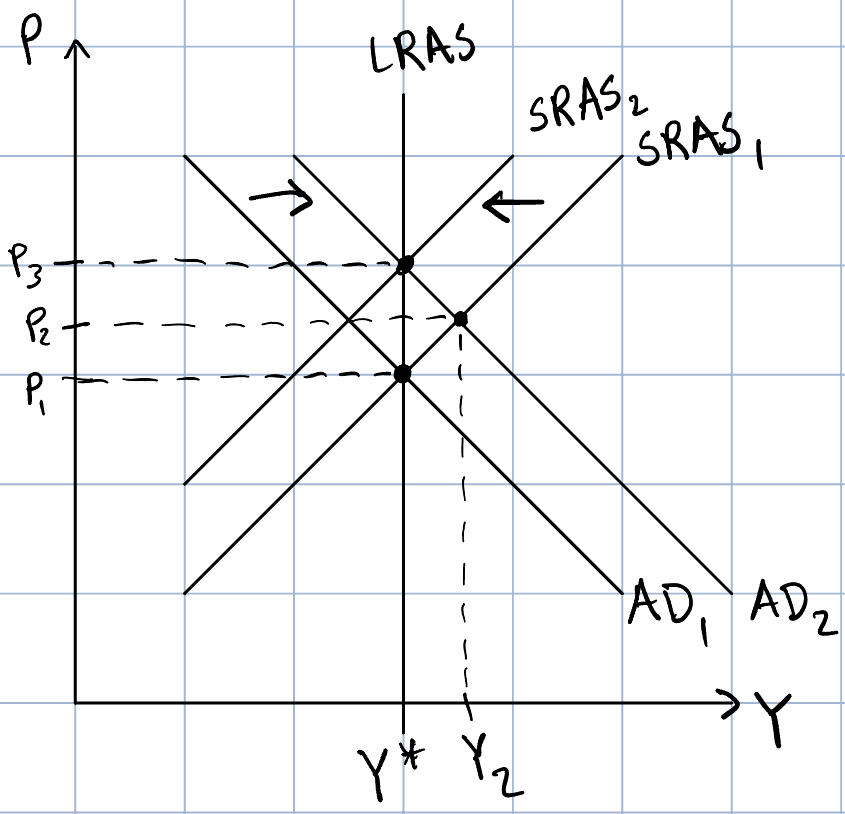
\includegraphics[width = 0.4\textwidth]{qq11}
	\end{center}
	
\item (c) -- Stagflation is the combination of a recession and inflation. That occurs when the SRAS curve shifts left.

	\begin{center}
	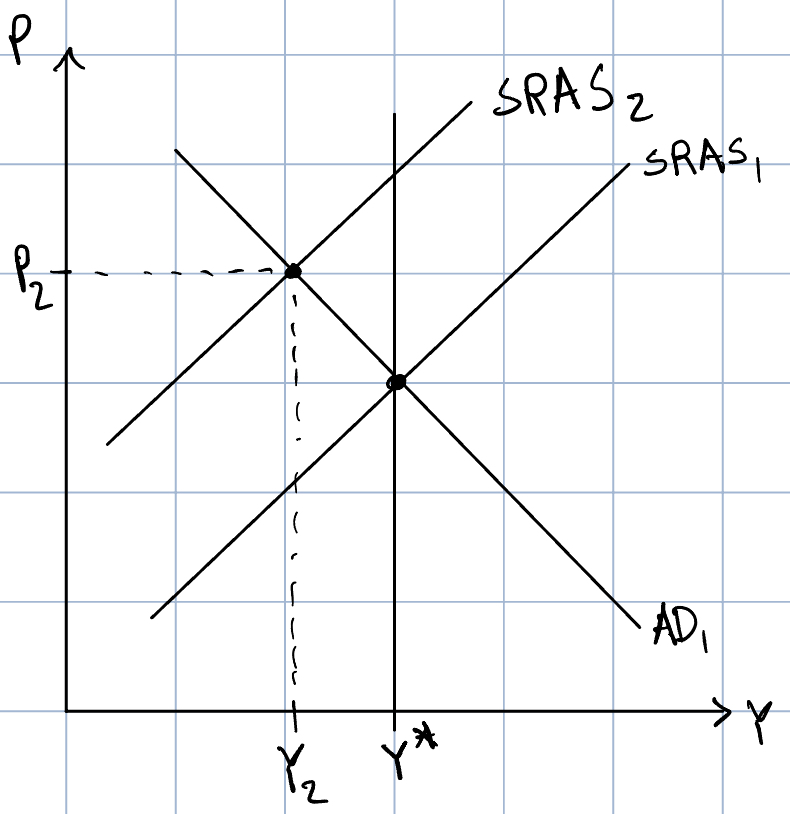
\includegraphics[width = 0.4\textwidth]{qq12}
	\end{center}

\end{enumerate}

\section*{Questions for Review}

\begin{enumerate}

\item Real GDP and investment decline when the economy goes into a recession. Unemployment rises when the economy goes into a recession.

\item \phantom{x}

	\begin{center}
	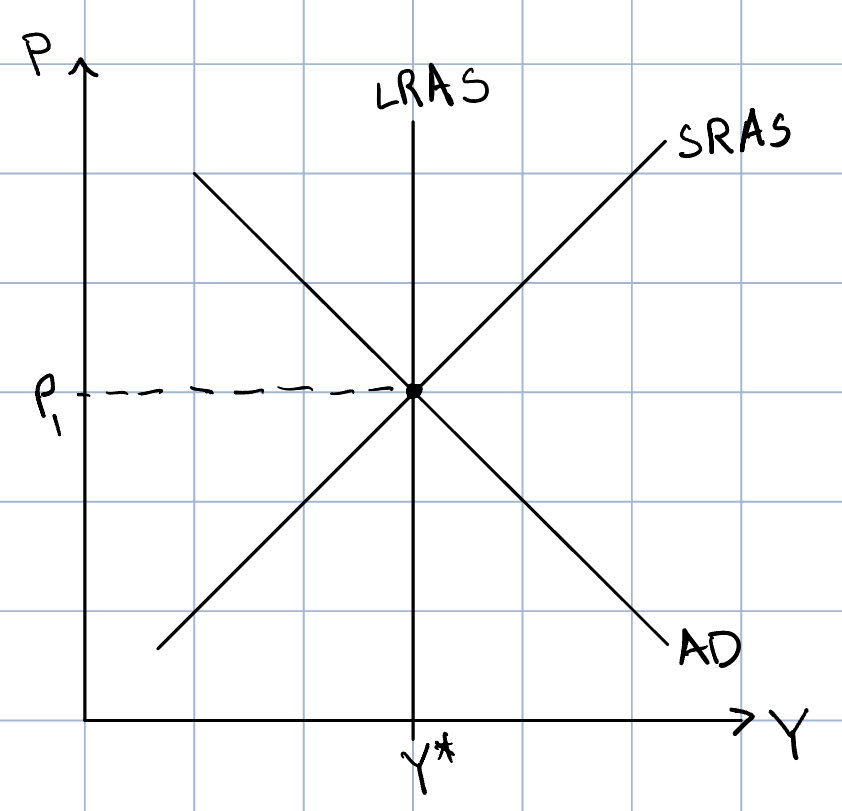
\includegraphics[width = 0.4\textwidth]{qfr2}
	\end{center}

\item

	\begin{itemize}
	
	\item The \underline{wealth effect}: When the price level decreases, the value of consumers' money increases, so consumers' become wealthier. In response to increased wealth, consumers consume more, so aggregate demand increases.
	
	\item The \underline{interest-rate effect}: When the price level decreases, the value of money increases, so people don't need to hold as much of it. That frees them up to lend more of their money, so the supply of loanable funds shifts to the right. As a result, investment increases and aggregate demand increases.
	
	\end{itemize}
	
\item The LRAS curve is vertical because the price level has no effect on output in the long run. In the long run, the determinants of output are capital (physical and human), natural resources, technological knowledge, and labor. The price level doesn't affect any of those determinants in the long run.
	
\item \begin{itemize}
	
	\item \underline{Sticky wages}: Firms and workers negotiate contracts that fix workers' nominal wages in the short-run. They negotiate based on what they expect the price level to be during the contract. If the actual price level turns out to be higher than expected during the contract, then the price of firms' output increases, but the workers' wages remain constant. That means the firms make higher profits than expected which incentivizes them to increase their production. Therefore, an increase in the price level causes an increase in production. 
		
	\item \underline{Sticky prices}: Firms set their prices based on what they expect the price level to be. If the actual price level turns out to be higher than expected, some firms won't immediately increase their prices because they'll be reluctant to pay the menu costs. As a result, those firms will have lower prices than the firms that do immediately respond, so those firms will have higher sales than expected. Higher sales will incentivize the firms to increase their production. Therefore, an increase in the price level causes an increase in production.
		
	\item \underline{Misperceptions}: If the price level moves higher than expected, some firms might misperceive it as an increase in the price of their particular output. That would make them think it had become more profitable to produce their good, so they would increase production. Therefore, an increase in the price level causes an increase in production.
	
	\end{itemize}
	
\item A stock market crash would decrease consumers' wealth. That would make them consume less and shift the AD curve to the left. In the short run, output and the price level would decrease. In the long run, SRAS would shift right, decreasing the price level further and returning the economy to its natural output level.

	\begin{center}
	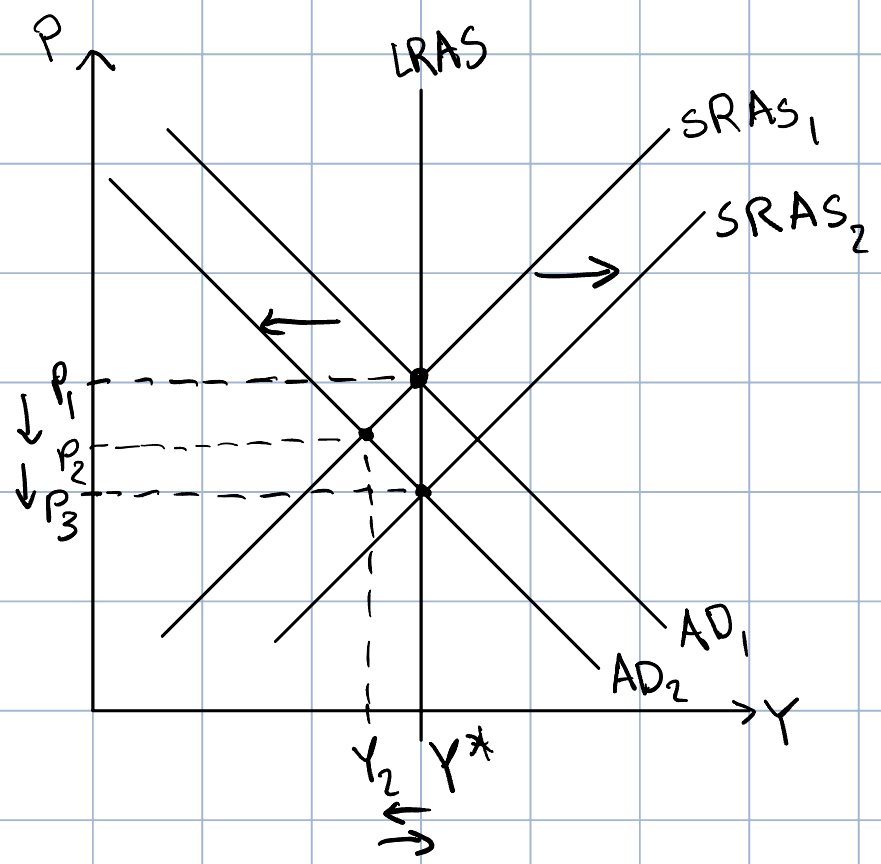
\includegraphics[width = 0.4\textwidth]{qfr6}
	\end{center}

\item Extreme weather that rendered some of the capital stock temporarily unusable would shift the aggregate-supply curve to the left. In the short run, output would decrease and the price level would increase. In the long run, the recession and inflation would worsen, but eventually the SRAS curve would shift right, and the economy would return to its original long-run equilibrium.

\end{enumerate}

\newpage

\section*{Problems and Applications}

\begin{enumerate}

\item

	\begin{enumerate}
	
	\item \phantom{x}
	
		\begin{center}
		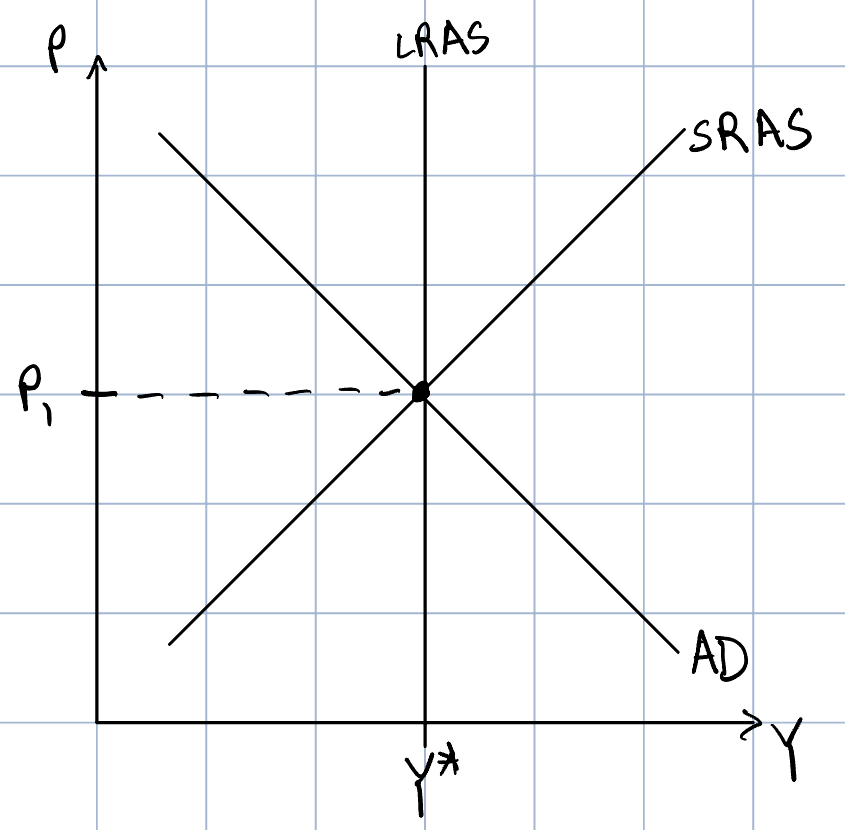
\includegraphics[width = 0.4\textwidth]{paa1a}
		\end{center}
	
	\item Output and the price level fall. Because output is below it's natural level, the economy is in a recession. During a recession, unemployment increases.
	
		\begin{center}
		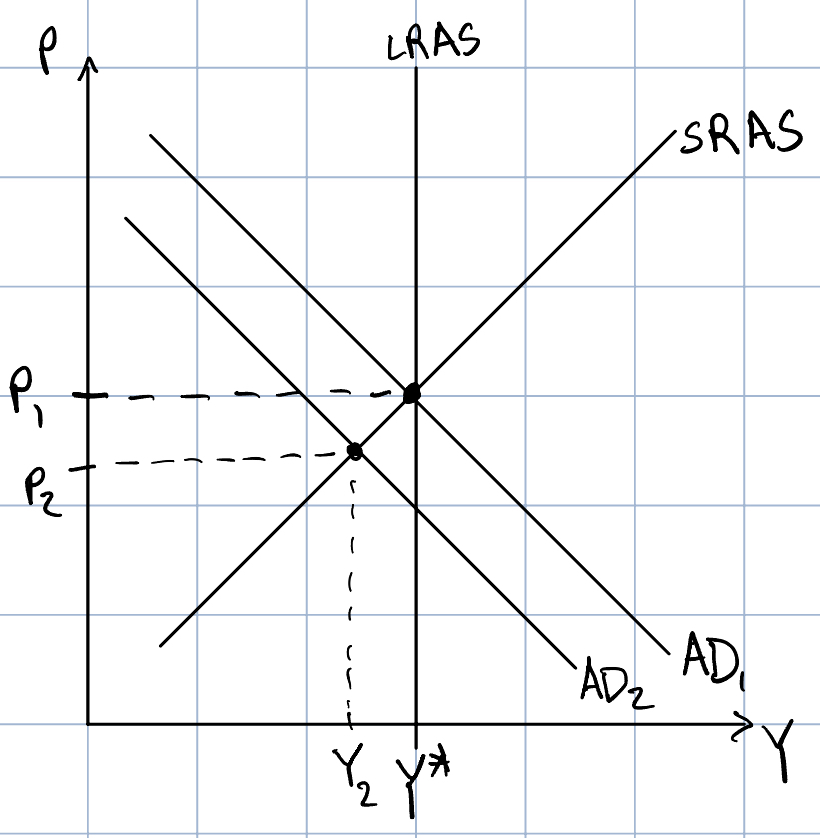
\includegraphics[width = 0.4\textwidth]{paa1b}
		\end{center}
	
	\item In the long run, firms and workers see that the price level has fallen, so they expect a lower price level than they did before the crash. Because they expect a lower price level, they will agree to lower wages than they did in the past. Firms are willing to pay less because the price of their output declines, and therefore their revenue declines. Workers will be willing to receive less because their cost of living is lower. As wages decrease, the cost of production decreases, so the aggregate supply curve shifts to the right. The economy returns to its natural output level at a lower price level.
	
		\begin{center}
		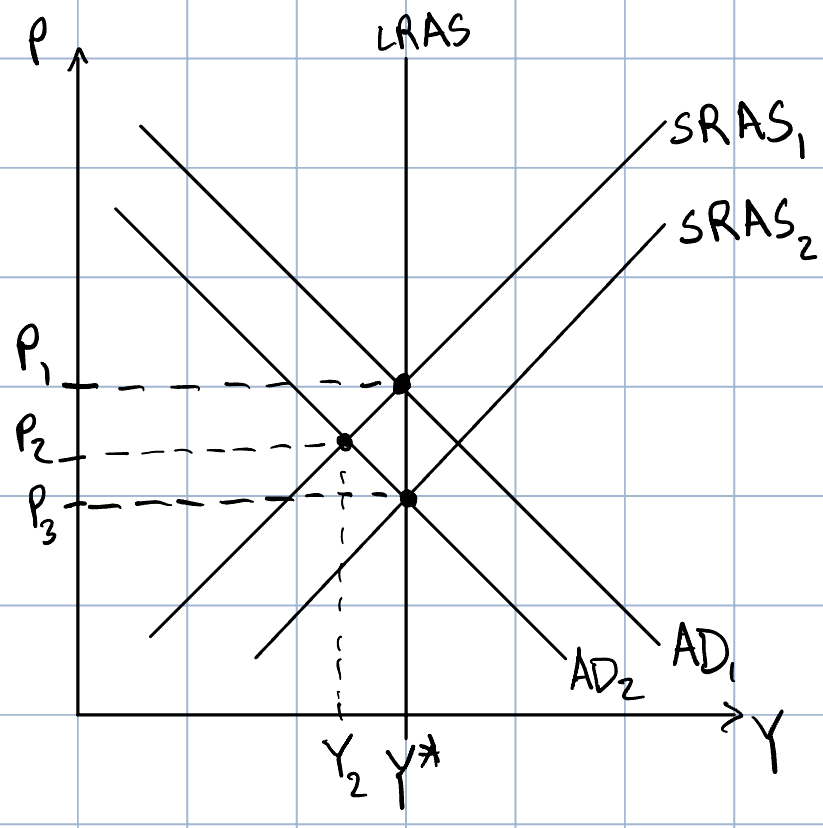
\includegraphics[width = 0.4\textwidth]{paa1c}
		\end{center}
	
	\end{enumerate}
	
\item

	\begin{enumerate}
	
	\item Aggregate supply increases because the amount of labor in the economy increases.

	\item If the labor market is perfectly competitive (an unlikely assumption), then the minimum wage will decrease employment. Less labor will decrease aggregate supply. You don't need to worry about this one.
	
	\item Aggregate supply increases because the country's technological knowledge increases.
	
	\item Aggregate supply decreases because the capital stock decreases.
	
	\end{enumerate}
	
\item

	\begin{enumerate}
	
	\item \phantom{x}
	
		\begin{center}
		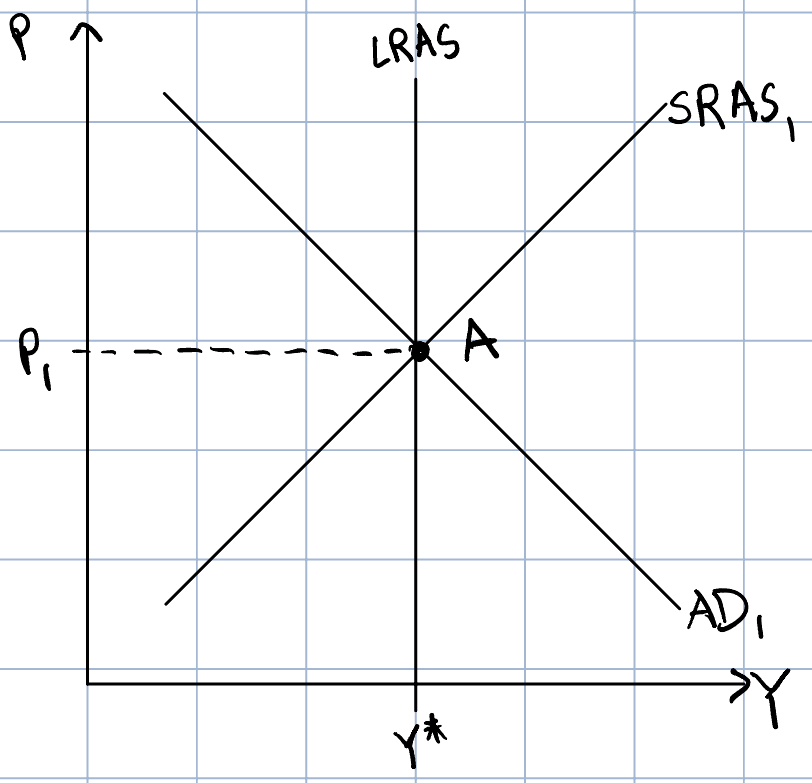
\includegraphics[width = 0.4\textwidth]{paa3a}
		\end{center}
	
	\item Output and the price level both increase.
	
		\begin{center}
		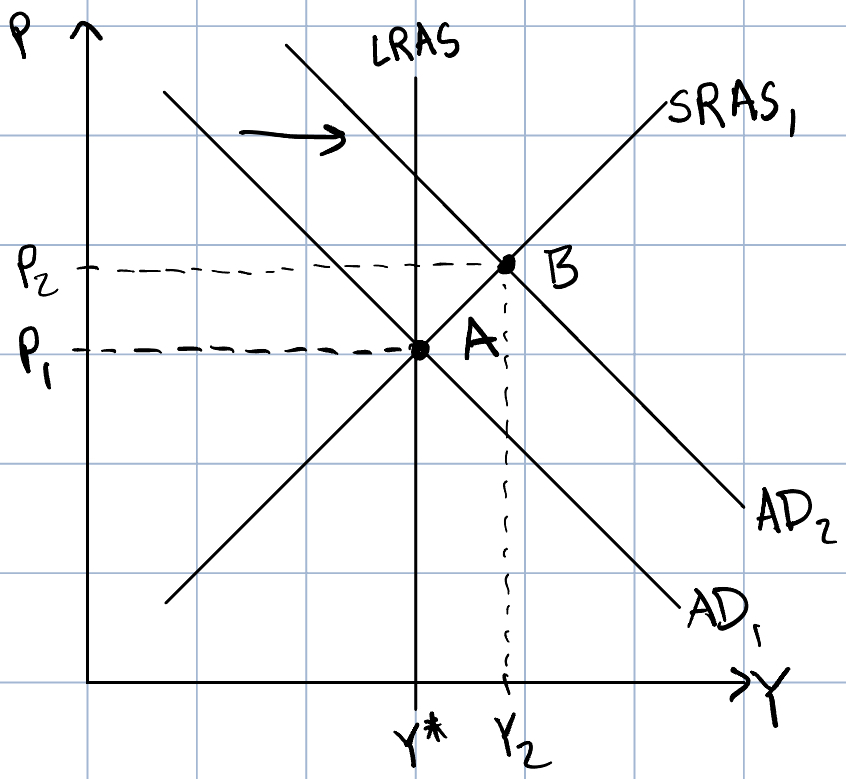
\includegraphics[width = 0.4\textwidth]{paa3b}
		\end{center}
		
	\item When the actual price level moves up, people begin to expect a higher price level than they did before the increase in the money supply. When the expected price level increases, the short-run aggregate supply curve shifts to the left. That moves the economy back to long-run equilibrium.
	
		\begin{center}
		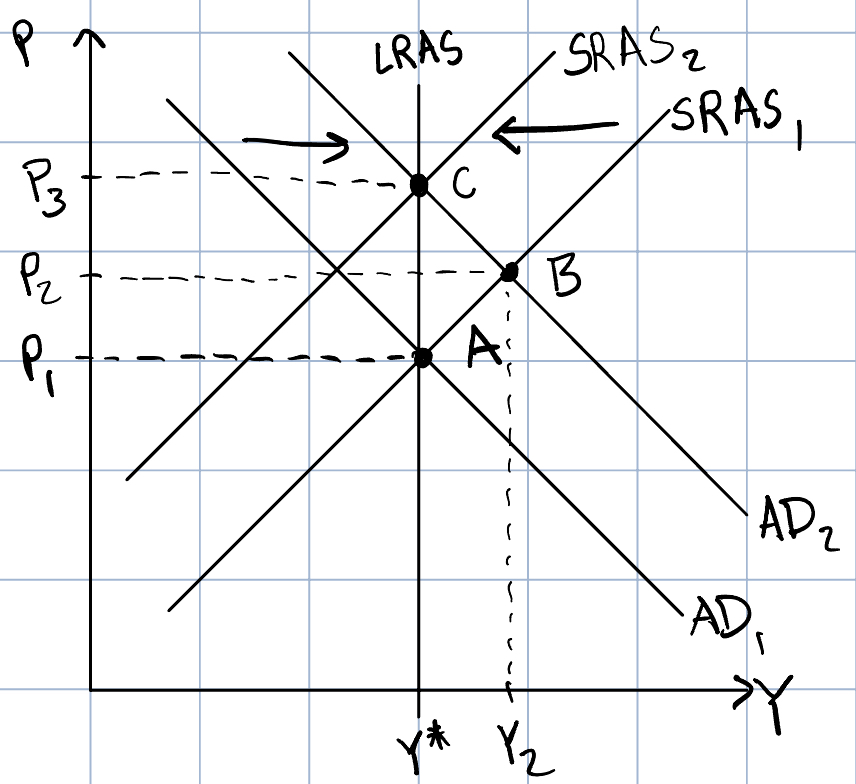
\includegraphics[width = 0.4\textwidth]{paa3c}
		\end{center}
		
	\item In the short run, nominal wages are fixed a.k.a. "sticky," so nominal wages are the same at point A and point B. In the long run, firms and workers expect a higher price level, so they negotiate new wages that account for those expectations. Firms are willing to pay more because they expect to receive more for their output, and workers demand more because they expect higher costs of living. 
	
	\item In the short run, nominal wages are fixed, so real wages decrease when the price level increases. Therefore, real wages decrease from A to B. In the long run, firms and workers re-negotiate wages to account for the higher price level, so real wages remain constant. Therefore, real wages are the same at A and C.
	
	\item It is. In the short run, an increase in the money supply increases real output and decreases real wages. In the long run, an increase in the money supply increases the price level but leaves real output and real wages unchanged.
	
	\end{enumerate}

\item If he wanted to lengthen the Christmas shopping period, he probably wanted to increase the amount of shopping households did. That means he wanted to increase consumption and shift the AD curve right. Since the economy was in a recession, a rightward shift in the AD curve would move the economy closer to natural output.

	\begin{center}
	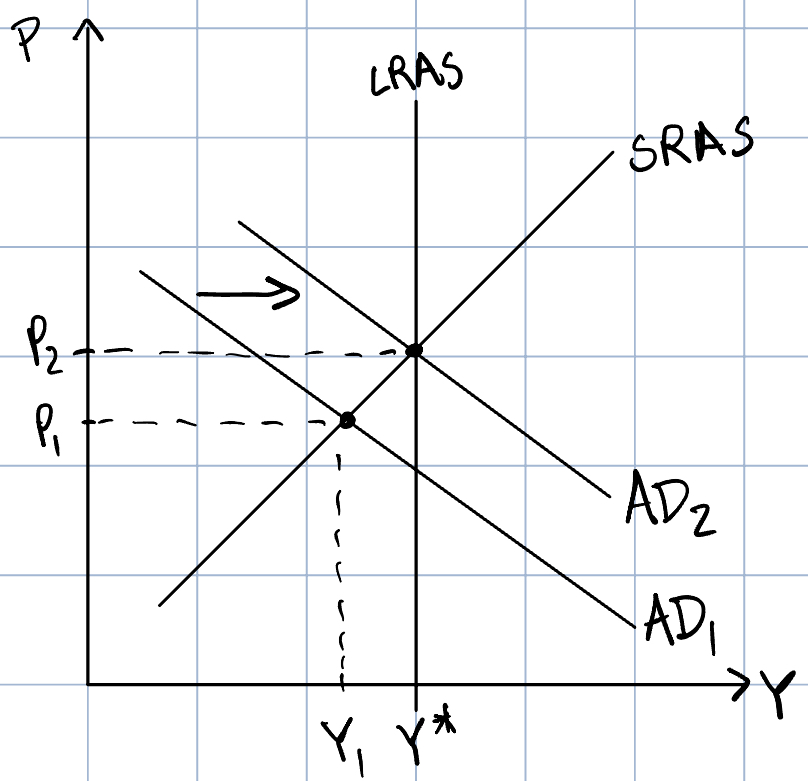
\includegraphics[width = 0.4\textwidth]{paa4}
	\end{center}
	
\item

	\begin{enumerate}
	
	\item The aggregate demand curve isn't the sum of the demand curves for different goods. That would give us the total number of goods demanded at any given price. We want the total output (a.k.a. GDP) at any given price level. Total output isn't the same as the total number of goods, and price isn't the same as price level.
	
	\item
	
	\end{enumerate}

\end{enumerate}

\end{document}